% figures/dispatch-path.tex
% The two launch dispatch lanes: compiled nanobind launcher and the
% ctypes fallback, both enqueueing on the current PyTorch stream.
\documentclass[tikz,border=10pt]{standalone}
% figures/common-preamble.tex
% Shared setup for the TikZ documentation figures. Colors mirror the
% palette in scripts/render_docs_diagrams.py so both atlases match.
\usepackage[T1]{fontenc}
\usepackage{lmodern}
\usepackage{tikz}
\usepackage{pgfplots}
\pgfplotsset{compat=1.18}
\usetikzlibrary{arrows.meta}
\usetikzlibrary{backgrounds}
\usetikzlibrary{calc}
\usetikzlibrary{decorations.pathreplacing}
\usetikzlibrary{fit}
\usetikzlibrary{positioning}

\definecolor{swcanvas}{HTML}{FFFDF8}
\definecolor{swpanel}{HTML}{F5F3ED}
\definecolor{swink}{HTML}{17212B}
\definecolor{swmuted}{HTML}{4B5563}
\definecolor{swline}{HTML}{59636E}
\definecolor{swblue}{HTML}{00689D}
\definecolor{swbluefill}{HTML}{DCEFFD}
\definecolor{swpurple}{HTML}{8E4775}
\definecolor{swpurplefill}{HTML}{F7E2EF}
\definecolor{sworange}{HTML}{A94500}
\definecolor{sworangefill}{HTML}{FCE5DC}
\definecolor{swgreen}{HTML}{00664B}
\definecolor{swgreenfill}{HTML}{DDF4EB}
\definecolor{swgrayfill}{HTML}{EEF0F2}

\pagecolor{swcanvas}
\AtBeginDocument{\color{swink}}

\tikzset{
  swcell/.style={
    draw, minimum width=0.46cm, minimum height=0.46cm, inner sep=0pt,
    line width=0.7pt, rounded corners=1pt},
  swbox/.style={
    draw=swline, fill=swpanel, rounded corners=6pt, line width=0.9pt},
  swarrow/.style={-{Stealth[length=6pt]}, draw=swline, line width=1pt},
  swtag/.style={
    draw, rounded corners=8pt, line width=0.9pt,
    font=\bfseries\scriptsize, inner xsep=8pt, inner ysep=4pt},
  swtitle/.style={anchor=west, font=\Large\bfseries, text=swink},
  swsubtitle/.style={anchor=west, font=\small, text=swmuted},
  swcode/.style={font=\small\ttfamily, text=swink},
  every picture/.style={line cap=round},
}

\begin{document}
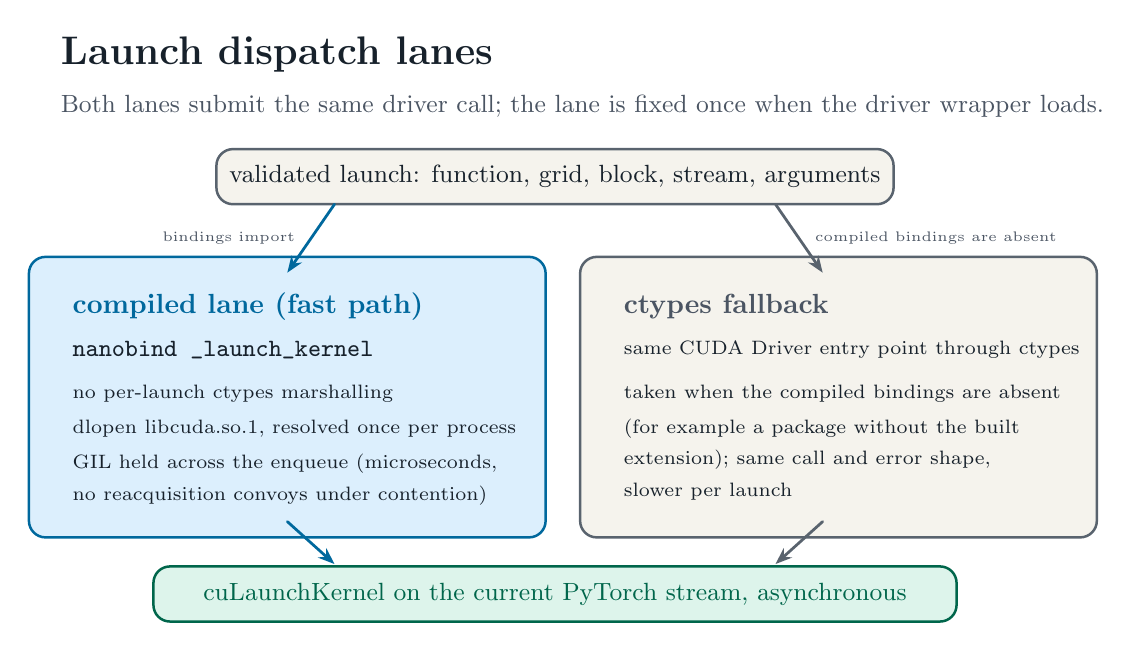
\begin{tikzpicture}[x=1cm, y=1cm]

% Header.
\node[swtitle] at (0, 1.15) {Launch dispatch lanes};
\node[swsubtitle] at (0, 0.5)
  {Both lanes submit the same driver call; the lane is fixed once
   when the driver wrapper loads.};

% The validated launch entering dispatch.
\node[swbox, minimum width=8.6cm, minimum height=0.7cm]
  (entry) at (6.4, -0.4) {};
\node[font=\small, text=swink] at (6.4, -0.4)
  {validated launch: function, grid, block, stream, arguments};

% Compiled lane.
\node[swbox, draw=swblue, fill=swbluefill,
      fit={(0, -4.7) (6.0, -1.7)}, inner sep=8pt] (native) {};
\node[anchor=west, font=\bfseries, text=swblue] at (0.15, -2.05)
  {compiled lane (fast path)};
\node[anchor=west, font=\small\ttfamily, text=swink] at (0.15, -2.6)
  {\detokenize{nanobind _launch_kernel}};
\node[anchor=west, font=\scriptsize, text=swink] at (0.15, -3.15)
  {no per-launch ctypes marshalling};
\node[anchor=west, font=\scriptsize, text=swink] at (0.15, -3.6)
  {dlopen libcuda.so.1, resolved once per process};
\node[anchor=west, font=\scriptsize, text=swink] at (0.15, -4.05)
  {GIL held across the enqueue (microseconds,};
\node[anchor=west, font=\scriptsize, text=swink] at (0.15, -4.45)
  {no reacquisition convoys under contention)};
\draw[swarrow, draw=swblue] (3.6, -0.75) -- (3.0, -1.62)
  node[midway, left=2pt, font=\tiny, text=swmuted]
  {bindings import};

% Fallback lane.
\node[swbox, fit={(7.0, -4.7) (13.0, -1.7)}, inner sep=8pt]
  (fallback) {};
\node[anchor=west, font=\bfseries, text=swmuted] at (7.15, -2.05)
  {ctypes fallback};
\node[anchor=west, font=\scriptsize, text=swink] at (7.15, -2.6)
  {same CUDA Driver entry point through ctypes};
\node[anchor=west, font=\scriptsize, text=swink] at (7.15, -3.15)
  {taken when the compiled bindings are absent};
\node[anchor=west, font=\scriptsize, text=swink] at (7.15, -3.6)
  {(for example a package without the built};
\node[anchor=west, font=\scriptsize, text=swink] at (7.15, -4.0)
  {extension); same call and error shape,};
\node[anchor=west, font=\scriptsize, text=swink] at (7.15, -4.4)
  {slower per launch};
\draw[swarrow] (9.2, -0.75) -- (9.8, -1.62)
  node[midway, right=2pt, font=\tiny, text=swmuted]
  {compiled bindings are absent};

% Both lanes reach the same asynchronous enqueue.
\node[swbox, draw=swgreen, fill=swgreenfill, minimum width=10.2cm,
      minimum height=0.7cm] (enqueue) at (6.4, -5.7) {};
\node[font=\small, text=swgreen] at (6.4, -5.7)
  {cuLaunchKernel on the current PyTorch stream, asynchronous};
\draw[swarrow, draw=swblue] (3.0, -4.78) -- (3.6, -5.32);
\draw[swarrow] (9.8, -4.78) -- (9.2, -5.32);

\end{tikzpicture}
\end{document}
